% SPDX-License-Identifier: CC-BY-SA-4.0
% Author: Matthieu Perrin
% Part: 
% Section: 
% Sub-section: 
% Frame: 

\begingroup

\begin{frame}{Programmation Multi-Threads: Théorie vs. Pratique}%{Du parallélisme à la concurrence}

  \on[y=-4.5mm]{
    \begin{tikzpicture}
      \begin{scope}
        \clip (-\paperwidth/2,0) rectangle (\paperwidth/2,7.5cm); 
        \node[anchor=south east, inner sep=0pt, outer sep=0pt] (parall) at (0,0) {
\includegraphics[width=\paperwidth/2]{pupies_theory}};
        \node[anchor=south west, inner sep=0pt, outer sep=0pt] (concur) at (0,0) {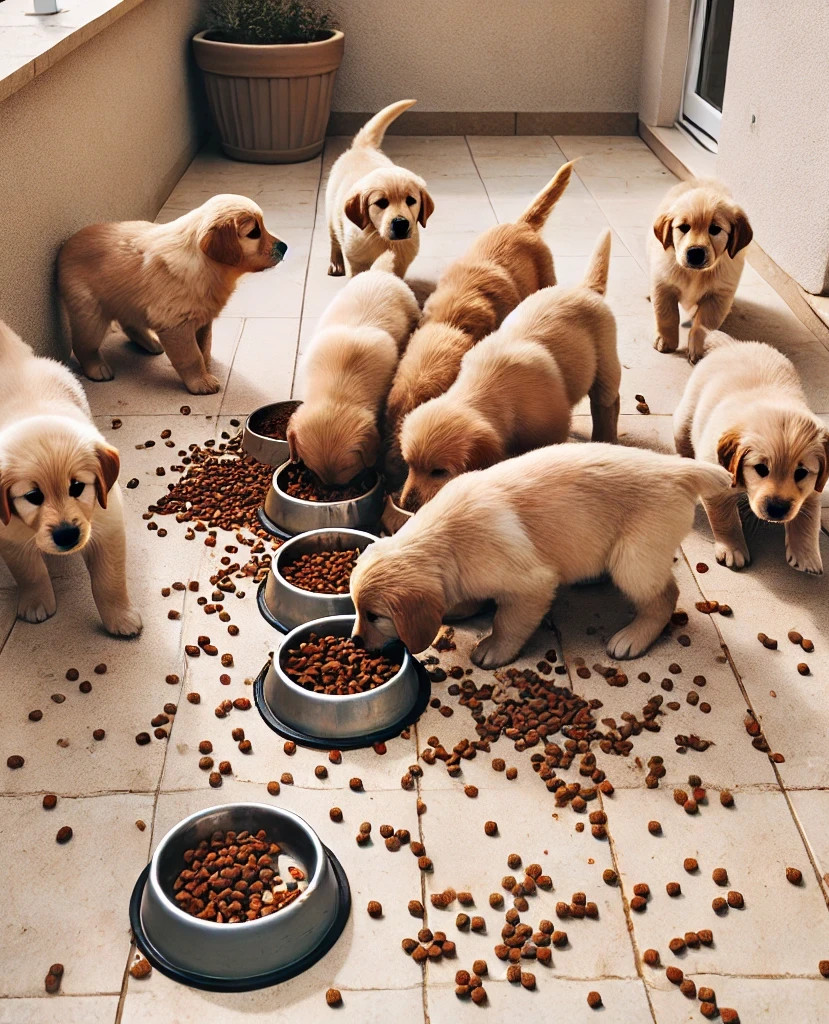
\includegraphics[width=\paperwidth/2]{pupies_practice}};
        \fill[white, path fading=south] (-\paperwidth/2,7.5cm) rectangle (\paperwidth/2,5cm); 
      \end{scope}
      \draw[white, thick] (-\paperwidth/2,7.5cm) -- (\paperwidth/2,7.5cm);
      \draw (0,0) -- (0,8cm);
      \fill[white, path fading=south] (-\paperwidth/2,8.01cm) rectangle (\paperwidth/2,7.5cm); 
      \draw (-\paperwidth/4,7.75cm) node{\Large Théorie : parallélisme} ;
      \draw ( \paperwidth/4,7.75cm) node{\Large Pratique : concurrence} ;
    \end{tikzpicture}
  }

\end{frame}

\endgroup
\endinput
